\documentclass[border=10pt]{standalone}
\usepackage{pgfplots}
\pgfplotsset{compat=1.17}
\begin{document}
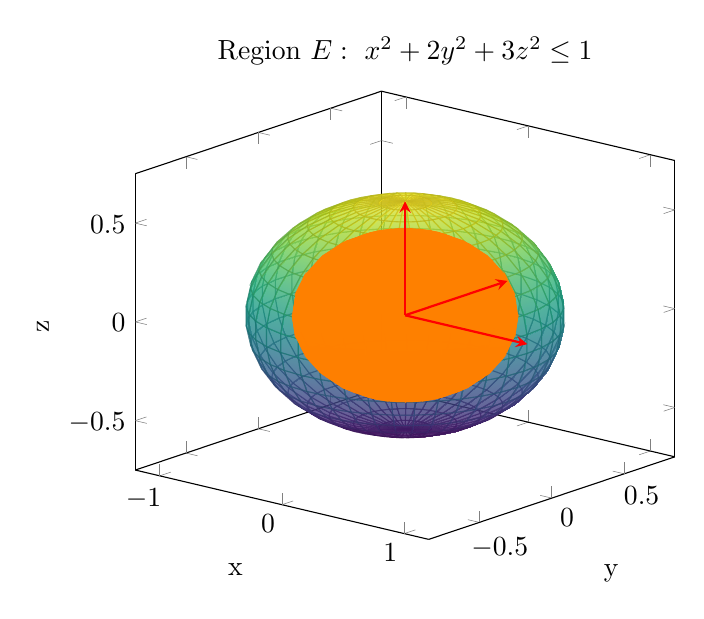
\begin{tikzpicture}
\begin{axis}[
    view={40}{20},
    xlabel={x}, ylabel={y}, zlabel={z},
    title={Region $E:\ x^2+2y^2+3z^2\le 1$},
    xmin=-1.2, xmax=1.2, ymin=-0.85, ymax=0.85, zmin=-0.75, zmax=0.75,
]
% outer boundary f = 0
\addplot3[surf, shader=faceted interp, colormap/viridis, opacity=0.55,
    domain=0:360, y domain=0:180, samples=40, samples y=20, z buffer=sort]
    ({cos(x)*sin(y)}, {sin(x)*sin(y)/sqrt(2)}, {cos(y)/sqrt(3)});
% inner level set f = 0.5
\addplot3[surf, shader=flat, color=orange, opacity=0.95,
    domain=0:360, y domain=0:180, samples=30, samples y=15, z buffer=sort]
    ({sqrt(0.5)*cos(x)*sin(y)}, {sqrt(0.5)*sin(x)*sin(y)/sqrt(2)}, {sqrt(0.5)*cos(y)/sqrt(3)});
% semi-axis rays
\addplot3[red, thick, -stealth] coordinates {(0,0,0) (1,0,0)};
\addplot3[red, thick, -stealth] coordinates {(0,0,0) (0,0.707,0)};
\addplot3[red, thick, -stealth] coordinates {(0,0,0) (0,0,0.577)};
\end{axis}
\end{tikzpicture}
\end{document}